\documentclass{article}

% if you need to pass options to natbib, use, e.g.:
%     \PassOptionsToPackage{numbers, compress}{natbib}
% before loading neurips_2019

% ready for submission
% \usepackage{neurips_2019}

% to compile a preprint version, e.g., for submission to arXiv, add add the
% [preprint] option:
%     \usepackage[preprint]{neurips_2019}

% to compile a camera-ready version, add the [final] option, e.g.:
%     \usepackage[final]{neurips_2019}

% to avoid loading the natbib package, add option nonatbib:
\usepackage[nonatbib, preprint]{neurips_2019}

\usepackage[utf8]{inputenc}           % allow utf-8 input
\usepackage[T1]{fontenc}              % use 8-bit T1 fonts
\usepackage{hyperref}                 % hyperlinks
\usepackage{url}                      % simple URL typesetting
\def\UrlBreaks{\do\/\do-}             % To properly break the long url
\usepackage{booktabs}                 % professional-quality tables
\usepackage{amsfonts}                 % blackboard math symbols
\usepackage{nicefrac}                 % compact symbols for 1/2, etc.
\usepackage{microtype}                % microtypography

\usepackage{setspace}                 % Double Spacing
\usepackage{lmodern}                  % Font-size setting
\usepackage{graphicx}                 % For Figures
\usepackage[labelfont=bf]{caption}    % For Figures' Caption
\usepackage[numbers,round]{natbib}    % For Citation

\title{Deep Learning-based Approach to Prediction of Volcanic Fallut Spread}

% The \author macro works with any number of authors. There are two commands
% used to separate the names and addresses of multiple authors: \And and \AND.
%
% Using \And between authors leaves it to LaTeX to determine where to break the
% lines. Using \AND forces a line break at that point. So, if LaTeX puts 3 of 4
% authors names on the first line, and the last on the second line, try using
% \AND instead of \And before the third author name.

\author{
  Hyecheol Jang \\
  Department of Computer Sciences\\
  University of Wisconsin–Madison\\
  Madison, WI 53706 \\
  \texttt{hyecheol.jang@wisc.edu} \\

  \And
  Kangwook Lee\thanks{Faculty Advisor} \\
  Department of Electrical and Computer Engineering \\
  University of Wisconsin–Madison\\
  Madison, WI 53706 \\
  \texttt{kangwook.lee@wisc.edu} \\
}

\begin{document}

\maketitle

\begin{abstract}
  \fontsize{11pt}{11pt} \selectfont {
    The abstract paragraph should be indented \nicefrac{1}{2}~inch (3~picas) on
    both the left- and right-hand margins. Use 10~point type, with a vertical
    spacing (leading) of 11~points.  The word \textbf{Abstract} must be centered,
    bold, and in point size 12. Two line spaces precede the abstract. The abstract
    must be limited to one paragraph.
  }
\end{abstract}

\begin{doublespacing}
\section{Introduction} % TODO Review Requested
\fontsize{11pt}{11pt} \selectfont {
  The volcanic eruption is one of the most severe natural disasters which occasionally happens.
  However, comparing to the other disasters which can be predicted, like typhoons and storms,
  predicting the exact time and scale of volcanic eruption considered as a very difficult task, 
  which might never be accurate, according to 
  Einarsson~\cite[as cited in][para.7 \& 30]{fountain_2015}. 
  Though there exist various ways that volcanic eruption to cause countless casualties and massive 
  economic loss, according to Yun~\cite[p.274]{Yun_2013}, the fallout ash, the focus of this 
  research, considered as one of the most significant by-products making deadly effects.
  Including the respiratory damage of lives, threatening the safety and reliability of air 
  transportation, and the collapse of structures caused by sedimentation of the ash, the fallout ash
  causes various impairments in a wide range of areas~\cite[p.274-275]{Yun_2013}.
  
  To mitigate the hazardous effects caused by the fallout ash, it is important to properly predict 
  the direction of ash spread and alert citizens who reside through the path of the ash dispersion. 
  Historically, by using the Eulerian or the Lagrangian approach, according to Bonadonna et al. 
  \cite[p.3-4]{Bonadonna2012}, scientists tried to make Volcanic Ash and Dispersion/Tracking 
  Model (VATDM). These models usually focused on predicting the pathway of fallout ash dispersion 
  and the amount of deposited ash while accepting limited variables~\cite[p.276]{Yun_2013}.

  However, these models’ predictability might be limited due to computing 
  performance~\cite[p.745-746]{Tanaka2022}, as the model needs to calculate the movement of all 
  particles that want to predict. To be more specific, the number of particles to be tracked by 
  VATDM and the calculation requirement have positive relationship; Scollo et al. 
  \cite{SCOLLO2011129} confirmed that it required up to hundreds of millions of particles to get 
  accurate simulation result, meaning that the simulation with small number of particles might not 
  able to illustrate the region of disperse accurately.

  To make a faster prediction, researchers studied on making a lighter and faster prediction model
  \cite{Searcy1998}, standardizing the eruption parameters required to run the model 
  (\cite[p.7]{Webley2009}), and figuring out the way to store and retrieve different kinds of data
  (satellite and prediction from the mathematical model), which needed when deciding the final 
  prediction result, more efficiently~\cite{Sorokin2016}. Though the advance of the models and 
  simulated results' utilization efficiency has been improved with the effort of numerous scholars, 
  still the needs of the calculation process last, which yet limiting the ability of prediction to 
  the computing power.

  \fontsize{10pt}{10.5pt} \selectfont{
    \begin{figure}
      \centering
      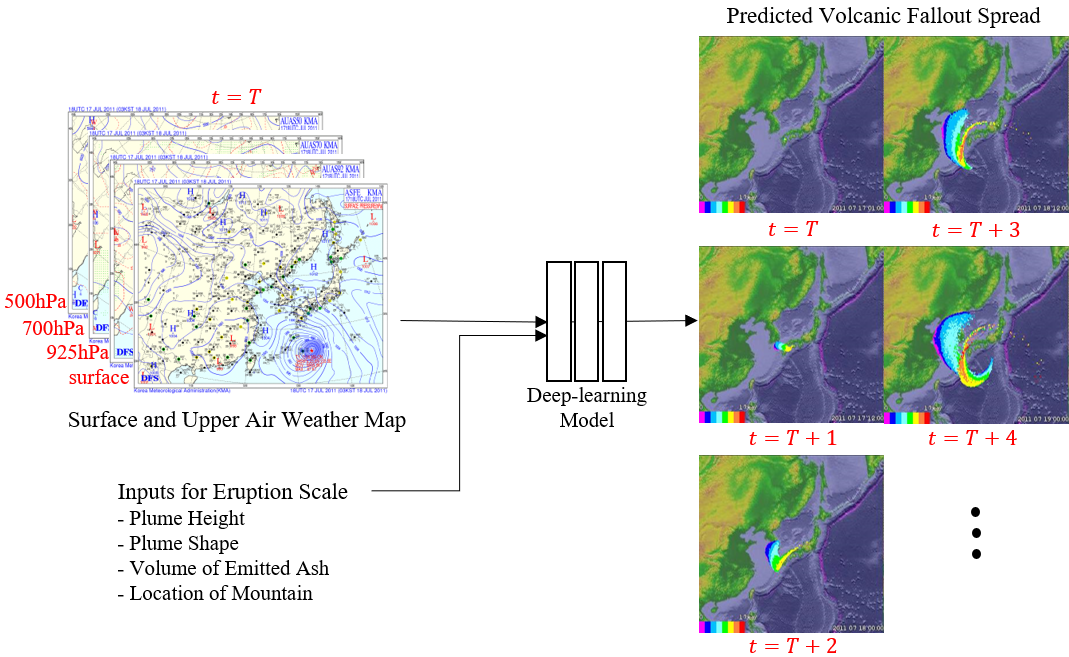
\includegraphics[width = \linewidth]{ModelStructure.png}
      \caption{\textbf{Overview of the Research Goal}
                This research aim to make a deep-learning model which predicts volcaninc fallout 
                spread while getting the weather maps (both surface and upper air) and eruption 
                scale parameters (Plume height, Plume shape, Volume of Emitted Ash, and the location
                of mountain) as an input.
              }
      \vspace{-5mm}
      \label{fig1}
    \end{figure}
  }

  In this research, we are going to suggest a faster way to get the prediction on the pathway and 
  area that might be affected by volcanic fallout ash: deep learning. By utilizing the
  state-of-the-arts deep learning architectures, our goal includes verifying whether deep learning 
  can predict the spread of fallout ash. (See \textbf{Figure \ref{fig1}} for the model's structure)

  To be more specific, we are going to construct a model based on the conditional Generative 
  Adversarial Network (cGAN), proposed by Isola et al. \cite{isola2016imagetoimage},which focused on
  translating one image to the other type of image (Image-to-Image Translation). Comparing to the 
  previous work \cite{isola2016imagetoimage}, while the previous architecture only got an image as 
  an input and produced one output image, our deep learning model should get several images and need
  to produce continous images to represent the direction and speed of ash spread. The details 
  regarding the model structure are writen below (Method - Model structure).
}

\section{Methods}  % TODO Review Requested
\fontsize{11pt}{11pt} \selectfont {
  \paragraph{Data Collection}
  To achieve our goal, making a generator which predicts the possible area of ash spread for the 
  given weather conditions and eruption scale, we first need to collect input and output data pairs.
  To collect these, for the input images, we will download those from the “Meteorological Data Open 
  Portal” operated by the Korea Meteorological Administration (KMA)~\cite[from][]{MDOP}. To get the
  output data, we will go through the traditional procedure (simulation with VATDM).
  
  The simulation parameters except for the weather data will be set manually. To represent various 
  eruption cases, for each mountain to be used as the sample, we will simulate with the constants 
  representing Volcanic Explosivity Index (VEI) 3 (Moderate Large Eruption), VEI 5 (Very Large 
  Eruption), and VEI 7 (Massive Explosive Eruption)~\cite[p.1232]{Newhall1982}. The weather 
  prediction data, will be obtained by the same location where we found the weather maps: download 
  prediction made by RDAPS(regional data assimilation and prediction system)~\cite[from][]{MDOP}.

  \paragraph{Model structure}
  We decide to use conditional GAN-based model, which has been shown to have good performance on 
  generating indistinguishable images compare to the \emph{real} images 
  \cite{isola2016imagetoimage}. The GAN has two distinctive parts of functions - Generator and 
  Discriminator - and we need to fit both function simultaneously. The goal for the Discriminator is
  to check whether the generated image is fake or not, while the Generator's goal is to make image, 
  which enough to make the Discriminator to categorize it to a \emph{real} image. While the original
  GAN only uses a random noize to generate the output, the conditional GAN not only gets random 
  noize but also gets the \emph{condition} vectors as an input. For our model, the condition vector 
  contains information of the weather maps and the eruption scale.

  Comparing our model with Isola et al.\cite{isola2016imagetoimage}'s cGAN model, whlie Isola et 
  al. provided only one image as an input, we have to pass not only the several weather map images 
  but also the numerical vector indicating the eruption scale of the volcano. Moreover, while Isola 
  et al.\cite{isola2016imagetoimage} challenged to provide randomness to their output, we want our 
  model to provide same output when the same inputs have been provided. Lastly, our model needs to 
  provide continuous images to represent the dispersion of volcaninc ash overtime, however, the 
  Isola et al.\cite{isola2016imagetoimage}'s model only need to provide a still photograph as an 
  output.

  To contruct the model, we will use U-Net architecture, proposed by proposed by Ronneberger et al.
  \cite{ronneberger2015unet}, for the convolutions to pass the information on the weather maps to 
  the neural network. As U-Net architecture has achieved a promising result on several different 
  image tasks\cite{isola2016imagetoimage,james2018simtoreal}, we are expecting that this 
  architecture also works for our task. However, we still have to come up with a solution to pass 
  information from several different images and one numerical vector to our neural network when we 
  train our model. After that, we are going to choose proper loss functions that make the best 
  result on predicting the relationship between elements depicted on the weather maps to the spread 
  of the ash.

  \paragraph{Model Analysis and Experiments}
  While we mauver over various loss functions, we are going to make various models utilizing 
  different loss functions and compare those with the quantitative metric. As indicated in the 
  previous paper \cite{isola2016imagetoimage}, it is difficult to say there exists one best 
  representation of the quality of translated images. Therefore, we need to set reliable 
  measurements before we analyze models using different loss functions.

  Once we decide the model structure, we need to verify the amount of sufficient size of training 
  datasets so that it can translate the weather map images to simulation results flawlessly. To do 
  these tasks, we need to train models with different amounts of inputs. As the Korean Peninsula 
  experiencing four distinctive seasons, while we picking up the training set randomly, we would 
  better ensure that we pick a combination of data that represents the dynamic climate of Korea. 
  After we fit the model with a different number of training datasets, we will investigate how well 
  each model draws the result.
}

\section{Timeline} % TODO Review Requested
\fontsize{11pt}{11pt} \selectfont {
  \fontsize{10pt}{10pt} \selectfont {
    \begin{table}
      \caption{Detailed Timeline}
      \label{table1}
      \centering
      \begin{tabular}{lll}
        \toprule
        \cmidrule(r){1-2}
        Due date     & Task description \\
        \midrule
        Mar. 14 & Select proper VATDM to generate training/testing sets \\ 
        Mar. 20 & Collect weather maps and weather prediction data \\
        Apr. 10 & Run simulation and collect outputs \\
        Apr. 31 & Choose candidates for final model's structure \\
        Jun. 15 & Conduct and analyze experiments on each nodels \\
        Jul. 15 & Write reports \\
        \bottomrule
      \end{tabular}
    \end{table}
  }

  The first thing we should do is to get the input. As there is no available API to get the weather 
  maps and data from KMA, but they provide an interactive website to download the data, it might 
  take some time to get all data manually. Moreover, the calculation time for that simulation was 
  not ignorable, according to a previous experiment (it takes approximately one hour to get one 
  output with the laptop having Intel’s i5-3320M CPU). Considering the factor that we have access to
  better computing power than the previous test, we are expecting to finish data collection within 
  two months after the project initiated.

  The next step is to train the generator with a given input-output pair. To fit the conditional GAN
  based model and to verify the result with various test cases, we are expecting to take two 
  additional months here. For the last month of this research, we will write a report and posters.

  The detailed timeline is on the \textbf{Table \ref{table1}}.
}

\section{Conclusion and Future Direction} % TODO Review Requested
\fontsize{11pt}{11pt} \selectfont {
  We are expected to make a deep neural network model to predict possible pathway and area of 
  volcanic fallout ash spread faster than the previous methods, by using simpler and lighter input, 
  weather maps, compare to the weather dataset predicted by RDAPS. Not only reduce the computing 
  time to predict the spread, but the model aims to reproduce as the same result as possible 
  compares to the original training result. To verify our idea and model structure, we utilize 
  weather maps representing the weather conditions and volcanos near the Korean Peninsula.
}

\end{doublespacing}

\medskip

\bibliography{reference}
\bibliographystyle{apalike}


\end{document}
